% Options for packages loaded elsewhere
\PassOptionsToPackage{unicode}{hyperref}
\PassOptionsToPackage{hyphens}{url}
%
\documentclass[
  11pt,
a4paper
]{article}

% Set up fonts
\usepackage[T1]{fontenc}
\usepackage[utf8]{inputenc}
\usepackage{amssymb,amsmath} % Need to load before unicode-math

% Customize floats: always put captions at the top and use the
% afore-defined typeface in tables. This packages also provides the
% `\floatfoot' environment for notes in floats.
\usepackage{floatrow}

% Make float numbers and labels stand out
\usepackage[labelfont=bf]{caption}

\usepackage{lmodern}
\usepackage{ifxetex,ifluatex}
\ifnum 0\ifxetex 1\fi\ifluatex 1\fi=0 % if pdftex
  \usepackage[T1]{fontenc}
  \usepackage[utf8]{inputenc}
  \usepackage{textcomp} % provide euro and other symbols
\else % if luatex or xetex
  \usepackage{unicode-math}
  \defaultfontfeatures{Scale=MatchLowercase}
  \defaultfontfeatures[\rmfamily]{Ligatures=TeX,Scale=1}
\fi

% Use upquote if available, for straight quotes in verbatim environments
\IfFileExists{upquote.sty}{\usepackage{upquote}}{}
\IfFileExists{microtype.sty}{% use microtype if available
  \usepackage[]{microtype}
  \UseMicrotypeSet[protrusion]{basicmath} % disable protrusion for tt fonts
}{}
\makeatletter
\@ifundefined{KOMAClassName}{% if non-KOMA class
  \IfFileExists{parskip.sty}{%
    \usepackage{parskip}
  }{% else
    \setlength{\parindent}{0pt}
    \setlength{\parskip}{6pt plus 2pt minus 1pt}}
}{% if KOMA class
  \KOMAoptions{parskip=half}}
\makeatother
\usepackage{xcolor}
\IfFileExists{xurl.sty}{\usepackage{xurl}}{} % add URL line breaks if available
\IfFileExists{bookmark.sty}{\usepackage{bookmark}}{\usepackage{hyperref}}
\hypersetup{
  pdftitle={Working Paper Template},
  pdfauthor={First Author; Second Author},
  pdfkeywords={Inequality, Intersectionality, Measurement, Poverty},
  hidelinks,
  pdfcreator={LaTeX via pandoc}}
\urlstyle{same} % disable monospaced font for URLs
\usepackage{geometry}

\usepackage{longtable,booktabs,array}
\usepackage{calc} % for calculating minipage widths

\usepackage[width=\textwidth]{caption}
% Make caption package work with longtable
\makeatletter
\def\fnum@table{\tablename~\thetable}
\makeatother

\usepackage{graphicx}
\makeatletter
\def\maxwidth{\ifdim\Gin@nat@width>\linewidth\linewidth\else\Gin@nat@width\fi}
\def\maxheight{\ifdim\Gin@nat@height>\textheight\textheight\else\Gin@nat@height\fi}
\makeatother
% Scale images if necessary, so that they will not overflow the page
% margins by default, and it is still possible to overwrite the defaults
% using explicit options in \includegraphics[width, height, ...]{}
\setkeys{Gin}{width=\maxwidth,height=\maxheight,keepaspectratio}
% Set default figure placement to htbp
\makeatletter
\def\fps@figure{htbp}
\makeatother
\renewcommand{\topfraction}{.85}
\renewcommand{\bottomfraction}{.7}
\renewcommand{\textfraction}{.15}
\renewcommand{\floatpagefraction}{.66}
\setcounter{topnumber}{3}
\setcounter{bottomnumber}{3}
\setcounter{totalnumber}{4}

\setlength{\emergencystretch}{3em} % prevent overfull lines
\providecommand{\tightlist}{%
  \setlength{\itemsep}{0pt}\setlength{\parskip}{0pt}}

\setcounter{secnumdepth}{3}

\usepackage{placeins}
\usepackage{flafter}
\usepackage{subfig}
\usepackage{booktabs}
\usepackage{longtable}
\usepackage{array}
\usepackage{multirow}
\usepackage{wrapfig}
\usepackage{float}
\usepackage{colortbl}
\usepackage{pdflscape}
\usepackage{tabu}
\usepackage{threeparttable}
\usepackage{threeparttablex}
\usepackage[normalem]{ulem}
\usepackage{makecell}
\usepackage{xcolor}
\ifluatex
  \usepackage{selnolig}  % disable illegal ligatures
\fi
\newlength{\cslhangindent}
\setlength{\cslhangindent}{1.5em}
\newlength{\csllabelwidth}
\setlength{\csllabelwidth}{3em}
\newenvironment{CSLReferences}[2] % #1 hanging-ident, #2 entry spacing
 {% don't indent paragraphs
  \setlength{\parindent}{0pt}
  % turn on hanging indent if param 1 is 1
  \ifodd #1 \everypar{\setlength{\hangindent}{\cslhangindent}}\ignorespaces\fi
  % set entry spacing
  \ifnum #2 > 0
  \setlength{\parskip}{#2\baselineskip}
  \fi
 }%
 {}
\usepackage{calc}
\newcommand{\CSLBlock}[1]{#1\hfill\break}
\newcommand{\CSLLeftMargin}[1]{\parbox[t]{\csllabelwidth}{#1}}
\newcommand{\CSLRightInline}[1]{\parbox[t]{\linewidth - \csllabelwidth}{#1}\break}
\newcommand{\CSLIndent}[1]{\hspace{\cslhangindent}#1}

\title{Working Paper Template\thanks{Thanks \ldots{}}}
\author{First Author\footnote{Institution, University, \href{mailto:email@address.com}{\nolinkurl{email@address.com}}} \and Second Author\footnote{Other Institution, Other University, \href{mailto:email@address.com}{\nolinkurl{email@address.com}}}}
\date{\today}



\begin{document}
% Create a fake title page because no reasonably long abstract will
% leave enough space at the bottom. And narrow the bottom margin to
% slide footnotes down. See Section 6.4 of the `geometry' package how
% they calculate the default 5.346cm.
\newgeometry{bottom=3cm}
\maketitle
\thispagestyle{empty} % Need to put after \maketitle
\begin{abstract}
  \noindent You can include the text for your abstract here.\\
  
  \noindent \textbf{JEL codes}: I24, I32, J15, J16
    
  \noindent \textbf{Keywords}: Inequality, Intersectionality, Measurement, Poverty
  \end{abstract}
\restoregeometry

\hypertarget{introduction}{%
\section{Introduction}\label{introduction}}

I can cite Illing et al. (2021) like this. I can also cite in parentheses (Illing et al., 2021).

The remainder of this paper proceeds as follows. Section \ref{background} introduces X. Section \ref{methods} describes the empirical strategy to estimate Y. Section \ref{data} presents more information on the data. Section \ref{results} presents the results of the analysis. Section \ref{conclusion} concludes.

The command \texttt{\textbackslash{}FloatBarrier} makes sure that floats such as tables and figures stay in their section.
\FloatBarrier 

\hypertarget{background}{%
\section{Background}\label{background}}

\FloatBarrier

\hypertarget{methods}{%
\section{Methodology}\label{methods}}

\FloatBarrier

\hypertarget{data}{%
\section{Data}\label{data}}

In many empirical papers you will have a Table One, aka a table with sample statistics or a balance table in case of an experimental paper. The easiest way is to use \texttt{gtsummary::tbl\_summary} to print a table with summary stats.

\begin{table}

\caption{\label{tab:summary1}Summary statistics with gtsummary}
\centering
\begin{tabular}[t]{ll}
\toprule
Characteristic & N = 32\\
\midrule
mpg & 19.2 (15.4, 22.8)\\
cyl & \\
\hspace{1em}4 & 11 (34\%)\\
\hspace{1em}6 & 7 (22\%)\\
\hspace{1em}8 & 14 (44\%)\\
\addlinespace
disp & 196 (121, 326)\\
hp & 123 (96, 180)\\
drat & 3.70 (3.08, 3.92)\\
\bottomrule
\multicolumn{2}{l}{\rule{0pt}{1em}\textsuperscript{1} Median (IQR); n (\%)}\\
\end{tabular}
\end{table}

At the moment the table caption appears below the table. I have not figured out yet why it does that.

We can also make a balance table.

\begin{table}

\caption{\label{tab:balance}A balance table using modelsummary}
\centering
\begin{tabular}[t]{llllllll}
\toprule
\multicolumn{2}{c}{ } & \multicolumn{2}{c}{0 (N=19)} & \multicolumn{2}{c}{1 (N=13)} & \multicolumn{2}{c}{ } \\
\cmidrule(l{3pt}r{3pt}){3-4} \cmidrule(l{3pt}r{3pt}){5-6}
  &    & Mean & Std. Dev. & Mean  & Std. Dev.  & Diff. in Means & Std. Error\\
\midrule
mpg &  & 17.1 & 3.8 & 24.4 & 6.2 & 7.2 & 1.9\\
disp &  & 290.4 & 110.2 & 143.5 & 87.2 & -146.8 & 35.0\\
hp &  & 160.3 & 53.9 & 126.8 & 84.1 & -33.4 & 26.4\\
drat &  & 3.3 & 0.4 & 4.0 & 0.4 & 0.8 & 0.1\\
wt &  & 3.8 & 0.8 & 2.4 & 0.6 & -1.4 & 0.2\\
qsec &  & 18.2 & 1.8 & 17.4 & 1.8 & -0.8 & 0.6\\
vs &  & 0.4 & 0.5 & 0.5 & 0.5 & 0.2 & 0.2\\
gear &  & 3.2 & 0.4 & 4.4 & 0.5 & 1.2 & 0.2\\
carb &  & 2.7 & 1.1 & 2.9 & 2.2 & 0.2 & 0.7\\
\midrule
 &  & N & \% & N & \% &  & \\
cyl & 4 & 3 & 15.8 & 8 & 61.5 &  & \\
 & 6 & 4 & 21.1 & 3 & 23.1 &  & \\
 & 8 & 12 & 63.2 & 2 & 15.4 &  & \\
\bottomrule
\multicolumn{8}{l}{\textsuperscript{} We can either add notes as part of the modelsummary/datasummary function call}\\
\end{tabular}
\floatfoot{\textbf{Notes:} Or as part of the floatfoot environment provided by the aswp package.} \end{table}



We can also generate a balance table using the \texttt{gtsummary} package, just as before

\begin{table}

\caption{\label{tab:balance2}Balance Table with gtsummary}
\centering
\begin{tabular}[t]{llll}
\toprule
Characteristic & 0, N = 19 & 1, N = 13 & p-value\\
\midrule
mpg & 17.3 (14.9, 19.2) & 22.8 (21.0, 30.4) & 0.002\\
cyl &  &  & 0.009\\
\hspace{1em}4 & 3 (16\%) & 8 (62\%) & \\
\hspace{1em}6 & 4 (21\%) & 3 (23\%) & \\
\hspace{1em}8 & 12 (63\%) & 2 (15\%) & \\
\addlinespace
disp & 276 (196, 360) & 120 (79, 160) & <0.001\\
hp & 175 (116, 192) & 109 (66, 113) & 0.046\\
drat & 3.15 (3.07, 3.70) & 4.08 (3.85, 4.22) & <0.001\\
wt & 3.52 (3.44, 3.84) & 2.32 (1.94, 2.78) & <0.001\\
qsec & 17.82 (17.18, 19.17) & 17.02 (16.46, 18.61) & 0.3\\
\addlinespace
vs & 7 (37\%) & 7 (54\%) & 0.3\\
gear &  &  & <0.001\\
\hspace{1em}3 & 15 (79\%) & 0 (0\%) & \\
\hspace{1em}4 & 4 (21\%) & 8 (62\%) & \\
\hspace{1em}5 & 0 (0\%) & 5 (38\%) & \\
\addlinespace
carb &  &  & 0.3\\
\hspace{1em}1 & 3 (16\%) & 4 (31\%) & \\
\hspace{1em}2 & 6 (32\%) & 4 (31\%) & \\
\hspace{1em}3 & 3 (16\%) & 0 (0\%) & \\
\hspace{1em}4 & 7 (37\%) & 3 (23\%) & \\
\addlinespace
\hspace{1em}6 & 0 (0\%) & 1 (7.7\%) & \\
\hspace{1em}8 & 0 (0\%) & 1 (7.7\%) & \\
\bottomrule
\multicolumn{4}{l}{\rule{0pt}{1em}\textsuperscript{1} Median (IQR); n (\%)}\\
\multicolumn{4}{l}{\rule{0pt}{1em}\textsuperscript{2} Wilcoxon rank sum test; Fisher's exact test; Pearson's Chi-squared test}\\
\multicolumn{4}{l}{\textsuperscript{a} We can also add footnotes here}\\
\end{tabular}
\end{table}

\FloatBarrier

\hypertarget{results}{%
\section{Results}\label{results}}

When we plot results the \texttt{floatfoot} environment allows us to add long notes to figures.



\begin{figure}
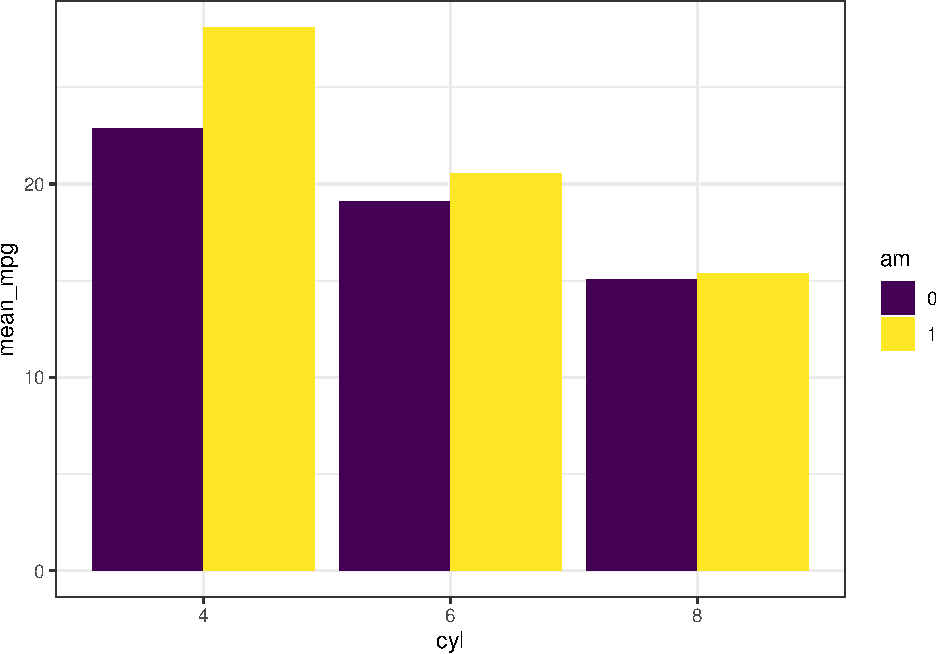
\includegraphics{figures/figure-1} \caption[A Figure]{A Figure}\label{fig:figure}
\floatfoot{\textbf{Notes:} Place the figure notes here to make sure they appear below the figure. I'm writing a bit more to show how nicely it works even with longer figure notes.} \end{figure}

We can also use modelsummary for regression tables.

\begin{table}

\caption{\label{tab:reg}Title for the table}
\centering
\begin{tabular}[t]{lcc}
\toprule
  & Model 1 & Model 2\\
\midrule
(Intercept) & 17.147*** & 29.004***\\
 & (0.880) & (1.491)\\
am1 & 7.245*** & 3.334***\\
 & (1.923) & (0.956)\\
cyl6 &  & -3.222**\\
 &  & (1.282)\\
cyl8 &  & -1.011\\
 &  & (2.633)\\
disp &  & -0.015\\
 &  & (0.010)\\
hp &  & -0.039***\\
 &  & (0.012)\\
\midrule
Num.Obs. & 32 & 32\\
R2 & 0.360 & 0.837\\
R2 Adj. & 0.338 & 0.806\\
se\_type & HC2 & HC2\\
\bottomrule
\multicolumn{3}{l}{\textsuperscript{} * p $<$ 0.1, ** p $<$ 0.05, *** p $<$ 0.01}\\
\multicolumn{3}{l}{\textsuperscript{} \emph{Notes:} I can add notes}\\
\multicolumn{3}{l}{\textsuperscript{} And even more notes if I want}\\
\end{tabular}
\floatfoot{(ref:note-reg)} \end{table}

\FloatBarrier

\hypertarget{conclusion}{%
\section{Conclusion}\label{conclusion}}

\clearpage

\hypertarget{references}{%
\section*{References}\label{references}}
\addcontentsline{toc}{section}{References}

\hypertarget{refs}{}
\begin{CSLReferences}{1}{0}
\leavevmode\hypertarget{ref-Illing2020}{}%
Illing, H., Schmieder, J., and Trenkle, S. (2021). \emph{{The Gender Gap in Earnings Losses after Job Displacement}}. \url{https://doi.org/10.3386/W29251}

\end{CSLReferences}

\appendix
\clearpage

\hypertarget{appendix-section}{%
\section{Appendix Section}\label{appendix-section}}

\FloatBarrier


\end{document}
